\documentclass{beamer}
\usepackage[utf8]{inputenc}
\usetheme{Copenhagen}
\usecolortheme{default}

\usepackage{graphicx}
\graphicspath{ {../Resources/} }

\title{An Introduction to Git and GitHub}
\author{Lan Peng}
\institute{Department of Industrial and Systems Engineering, University at Buffalo, SUNY}
\date{\today}

\begin{document}
	\frame{\titlepage}
	
	\begin{frame}
		\frametitle{Outline}
		\tableofcontents
	\end{frame}

	\section{Version control and Git}
		\subsection{Version control}
			\begin{frame}
				\frametitle{Version Control}
				\begin{align}
					\centering
					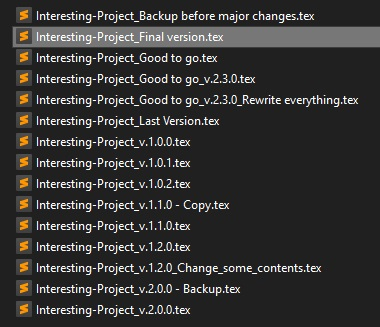
\includegraphics[height=6cm]{version_control} \nonumber
				\end{align}			
			\end{frame}

			\begin{frame}
				\frametitle{Version Control}
				The disadvantage of control version in this way
				\begin{itemize}
					\item Too messy, hard to find the latest (time stamps sometimes can't help)
					\item Cannot compare the difference between each version
					\item 
				\end{itemize}
			\end{frame}
		\subsection{What do we need for Version control?}
		\subsection{Git}
			\begin{frame}
				Solution: Git
			\end{frame}

	\section{Git and GitHub}
		\subsection{Installation Git}
			\begin{frame}
				\frametitle{Installation}
				\begin{itemize}
					\item Windows: \url{https://git-scm.com/downloads}
					\item Linux: \texttt{sudo apt-get install git}
					\item Mac OS: 
						\begin{enumerate}
							\item Install \texttt{Xcode} from AppStore 
							\item Run \texttt{Xcode} 
							\item In \texttt{Xcode -> Preferences} find \texttt{Downloads} 
							\item Choose \texttt{Command Line Tools}, install it
						\end{enumerate}					
				\end{itemize}
			\end{frame}

			\begin{frame}
				\frametitle{Installation}
				After installation, open the terminal and input \texttt{git} to see if it is successfully installed. There should be something like this:
				\begin{align}
					\centering
					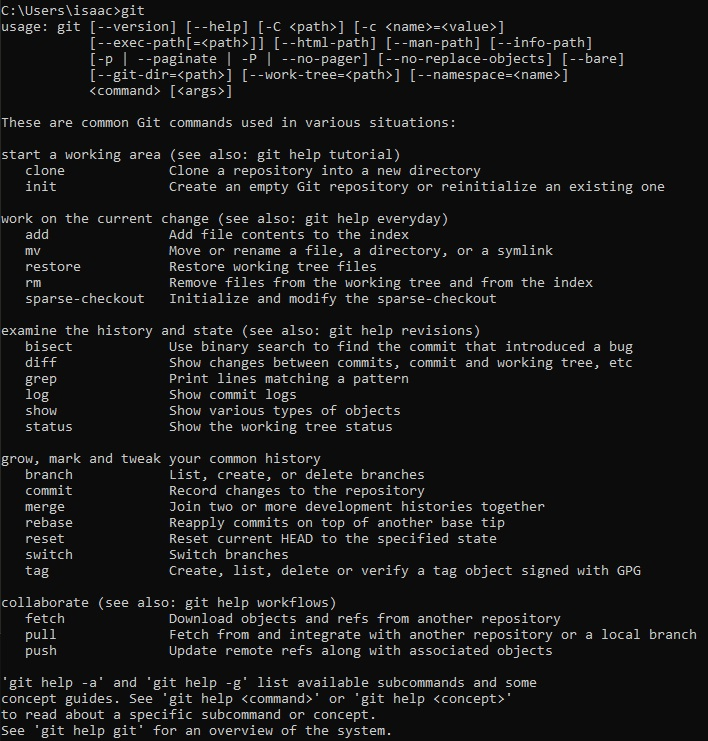
\includegraphics[height=5cm]{git_installed} \nonumber
				\end{align}
			\end{frame}
		\subsection{What is GitHub}
			\begin{frame}
				\frametitle{GitHub}
				\begin{itemize}
					\item A/the global company that provides hosting for software development version control using Git
					\item A website Microsoft just bought for \$7.5 billion dollar
					\item A website that you can goof around when you are bored at coding and don't need to worry about getting caught by your manager (she/he might be doing the same thing)
				\end{itemize}
			\end{frame}

			Test

	\section{Using Git and GitHub}
		\subsection{Initialize/Clone}
			\begin{frame}
				\frametitle{Initialize/Clone}
				\begin{itemize}
					\item \texttt{git init}
				\end{itemize}
				Create a \texttt{.git} folder in current path, making current path a git repository

				\begin{itemize}
					\item \texttt{git clone}
				\end{itemize}
				From a remote repository clone to current path
			\end{frame}

		\subsection{Branch}
			\begin{frame}
				\frametitle{Branch}
			\end{frame}

		\subsection{Commit}
			\begin{frame}
				\frametitle{Commit}
				\begin{itemize}
					\item Step 0: Check changes using \texttt{git status}
					\item Step 1: Add changes
				\end{itemize}
			\end{frame}

		\subsection{Merge}
			\begin{frame}
				\frametitle{Merge}
				\begin{itemize}
					\item Step 1. Go to the branch you need to merge into (e.g. master)
					\item Step 2. \texttt{git merge <branch>}
				\end{itemize}
			\end{frame}

			\begin{frame}
				\frametitle{Conflict}
				When could be conflict?
				\begin{itemize}
					\item 
				\end{itemize}
			\end{frame}

			\begin{frame}
				\frametitle{Tip}
				We don't like to merge changes in the same file, here are some tips to avoid that:
				\begin{itemize}
					\item Design by module. Each group member works on separated file, have someone (e.g., team leader) design the interface between modules
					\item Sync with master branch more often
					\item Commit with small changes (it depends)
				\end{itemize}
			\end{frame}

		\subsection{Revert/Reset}

		\subsection{.gitignore}

		\subsection{Pull request}

\end{document}